\documentclass[10pt,a4paper]{article}
\usepackage[margin=2cm]{geometry}
\usepackage{amsmath,amssymb,graphicx,caption,float,hyperref,xcolor}
\hypersetup{colorlinks=true,linkcolor=blue!50!black,urlcolor=blue!50!black}
\captionsetup{font=small,labelfont=bf}
\graphicspath{{../../figures/}}
\title{\vspace{-1.2cm}\textbf{Reading reversal and persistence: what the existing data show}\\[2pt]
\large Simulation 2, \texttt{task003-symmetric} and \texttt{task003-nosolution}}
\author{Step 1 of the key-phenomena study; 20 October 2026; no new simulations}
\date{}
\begin{document}
\maketitle
\vspace{-1cm}

\paragraph{Setting and notation.} Main setting: $q_c = 12$, $\lambda_c = 1$, vote gate on, budget $B = 30$, window
$W = 48$, 1{,}000 paired episodes per setting. $G$: paired susceptibility of the false controller (target A2), i.e.\
the mean over episodes of the A2 vote share with the controller minus the same episode's share without it.
$D(q_1\!\to\!q_2) = G(q_2) - G(q_1)$, computed per episode: episodes are paired across $q$ because every random stream
is keyed by seed, episode and purpose, never by $q$. $\delta(s)$: the paired effect $s$ time units after the
controller's last post $t^*$. Bars and bands: 95\% intervals. Details and tables: \texttt{02\_reanalysis\_existing\_data.md}.

%-----------------------------------------------------------------------------------------------------------------------
\section{The reading reversal}

\begin{figure}[H]
\centering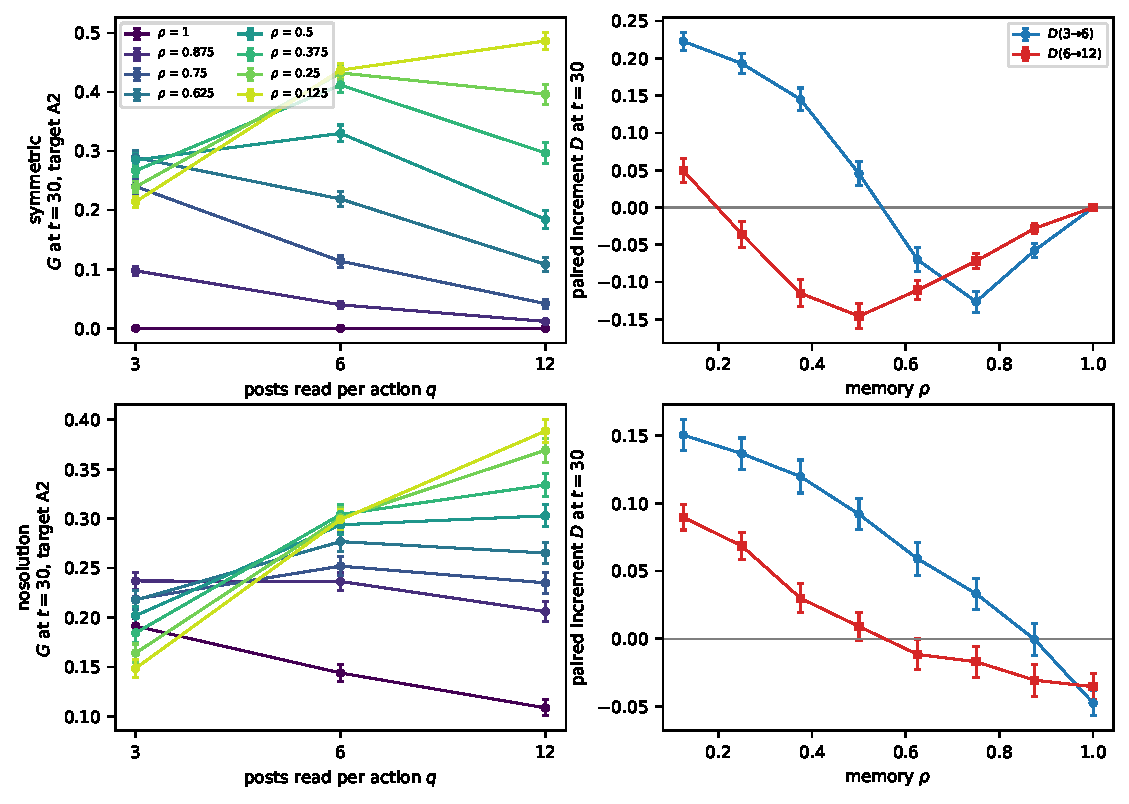
\includegraphics[width=0.95\linewidth]{fig1_reversal_map.pdf}
\caption{Left: $G$ at $t = 30$ against the posts each agent reads, $q$, one line per memory $\rho$. Right: the paired
increments $D(3\!\to\!6)$ and $D(6\!\to\!12)$ against $\rho$. Top: symmetric; bottom: nosolution.}
\label{fig:map}
\end{figure}

\begin{itemize}\itemsep1pt
\item Reading more helps the false controller when agents forget and protects the swarm when they remember, in both
  tasks.
\item Each step of $q$ changes sign at a different memory: symmetric $\rho \approx 0.55$ ($3\!\to\!6$) and $\approx 0.20$
  ($6\!\to\!12$); nosolution $\approx 0.87$ and $\approx 0.55$. The crossover is a sloped contour in $(\rho, q)$, about
  0.33 higher in $\rho$ without a proof.
\item The controller's best $q$ falls as memory grows (symmetric: 12, then 6, then 3; nosolution likewise, shifted to
  higher $\rho$).
\item Nosolution at $\rho = 0.75$: $G$ peaks at $q = 6$ ($D(3\!\to\!6) = +0.033 \pm 0.011$, $D(6\!\to\!12) = -0.017 \pm 0.011$).
\item The signs hold across all 72 combinations of $q_c$, rate and gate, and with $W = 24$, $W = 240$ and $B = 100$,
  except inside the crossover cells.
\end{itemize}

\begin{figure}[H]
\centering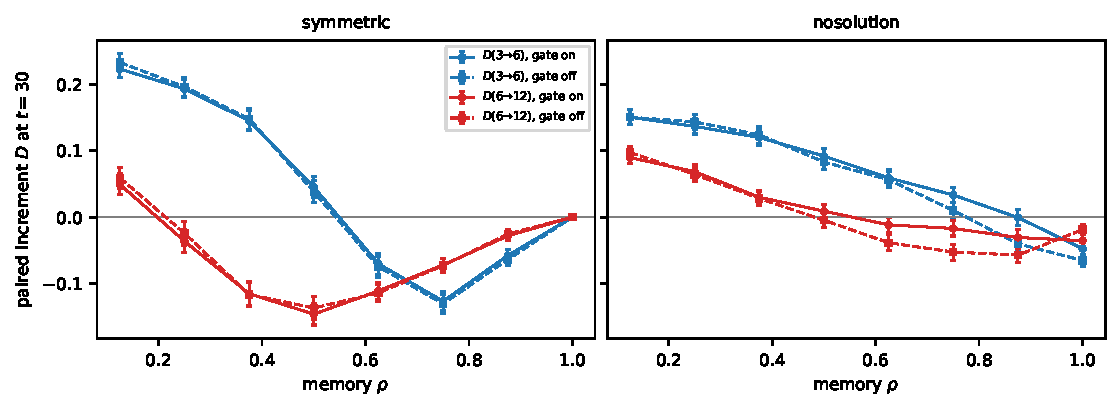
\includegraphics[width=0.95\linewidth]{fig4_dose.pdf}
\caption{$D(3\!\to\!6)$ and $D(6\!\to\!12)$ at $t = 30$ with the vote gate on (solid) and off (dashed). With the gate
off the controller posts 27.9 messages at every $q$.}
\label{fig:dose}
\end{figure}

\begin{itemize}\itemsep1pt
\item At equal dose (gate off) the increments keep their sign wherever it is clear and change by at most 0.04: the
  reversal is not a dose effect.
\end{itemize}

\begin{figure}[H]
\centering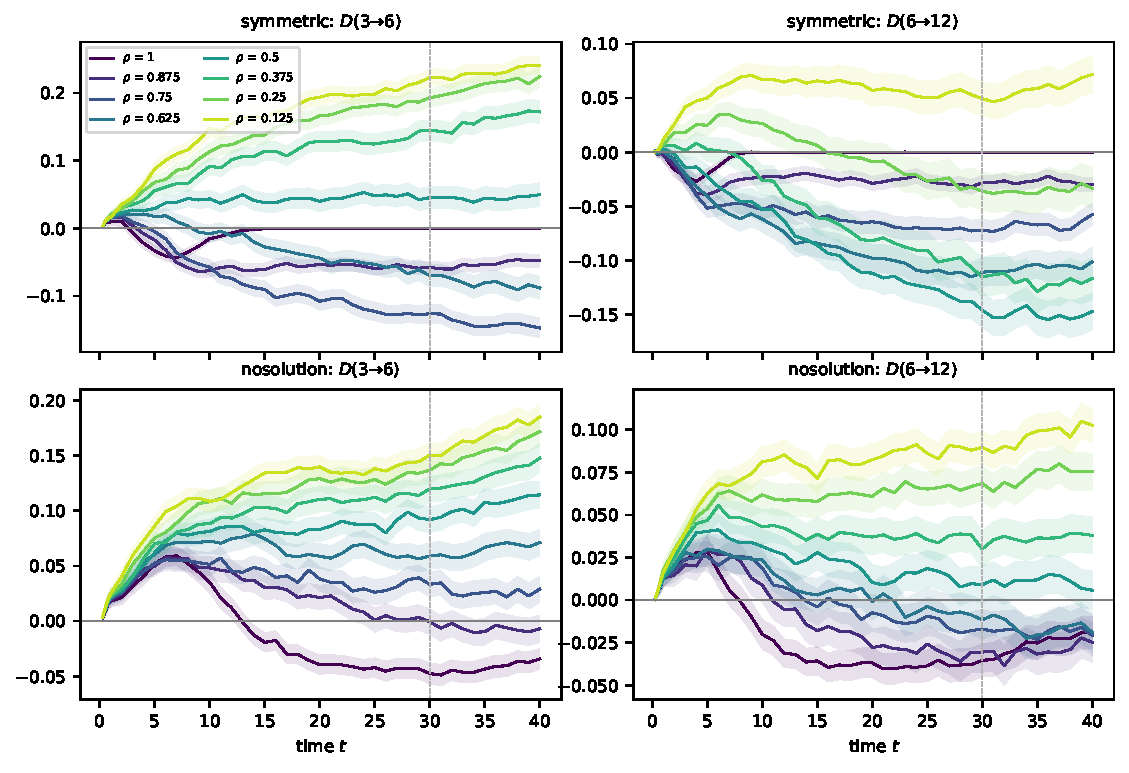
\includegraphics[width=0.95\linewidth]{fig2_reversal_time.pdf}
\caption{$D(3\!\to\!6)$ and $D(6\!\to\!12)$ over time, one line per $\rho$; the controller stops at $t = 30$ (dashed).}
\label{fig:time}
\end{figure}

\begin{itemize}\itemsep1pt
\item At $t = 2$ every increment is positive (except symmetric $D(6\!\to\!12)$ at $\rho \ge 0.5$, $\ge -0.016$): reading
  first spreads the controller's facts faster.
\item The protective sign builds up over tens of time units, e.g.\ nosolution $\rho = 1$, $D(3\!\to\!6)$: $+0.052$ at
  $t = 5$, $-0.047$ at $t = 30$.
\end{itemize}

%-----------------------------------------------------------------------------------------------------------------------
\section{What agents remember and what the board carries}

\begin{figure}[H]
\centering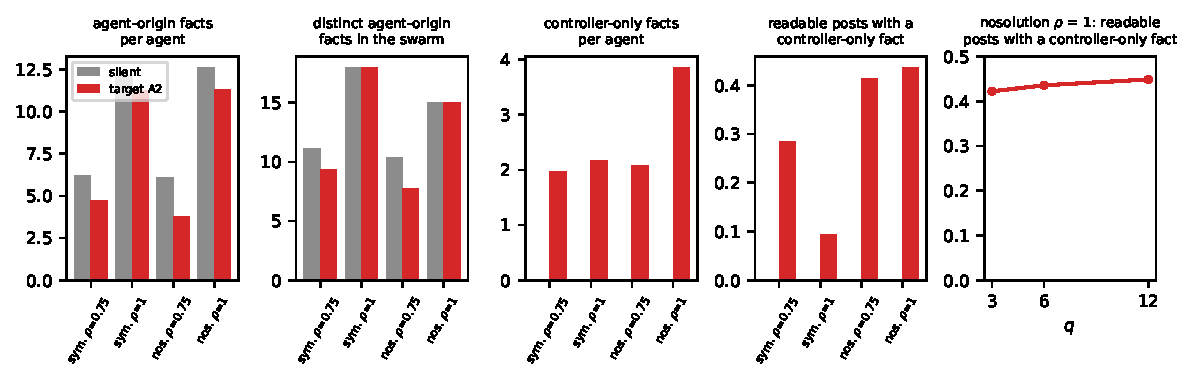
\includegraphics[width=0.98\linewidth]{fig5_mechanism.pdf}
\caption{Full records ($q = 6$, $\lambda_c = 1$, $t = 30$): silent (grey) against the false controller (red), for
symmetric and nosolution at $\rho = 0.75$ and 1. Right: nosolution, $\rho = 1$, readable posts with a controller-only
fact against $q$ (seed 2027, posts only).}
\label{fig:mech}
\end{figure}

\begin{itemize}\itemsep1pt
\item The controller crowds out the agents' own evidence: at $\rho = 0.75$ agents remember 1.5--2.3 fewer
  agent-origin facts and the swarm holds 1.8--2.6 fewer distinct ones.
\item At $\rho = 1$ every agent fact is held by someone in both arms (18/18, 15/15); in symmetric this is a proof and
  $G = 0$.
\item Controller-only facts make up 29--44\% of readable posts, except symmetric $\rho = 1$ (10\%).
\item Nosolution $\rho = 1$: the controller-only share of the board rises slightly with $q$ (0.42 $\to$ 0.45) while $G$
  falls (0.19 $\to$ 0.11). The protection is not on the board; memory records across $q$ are needed (step 2).
\end{itemize}

%-----------------------------------------------------------------------------------------------------------------------
\section{Persistence after the controller stops}

\begin{figure}[H]
\centering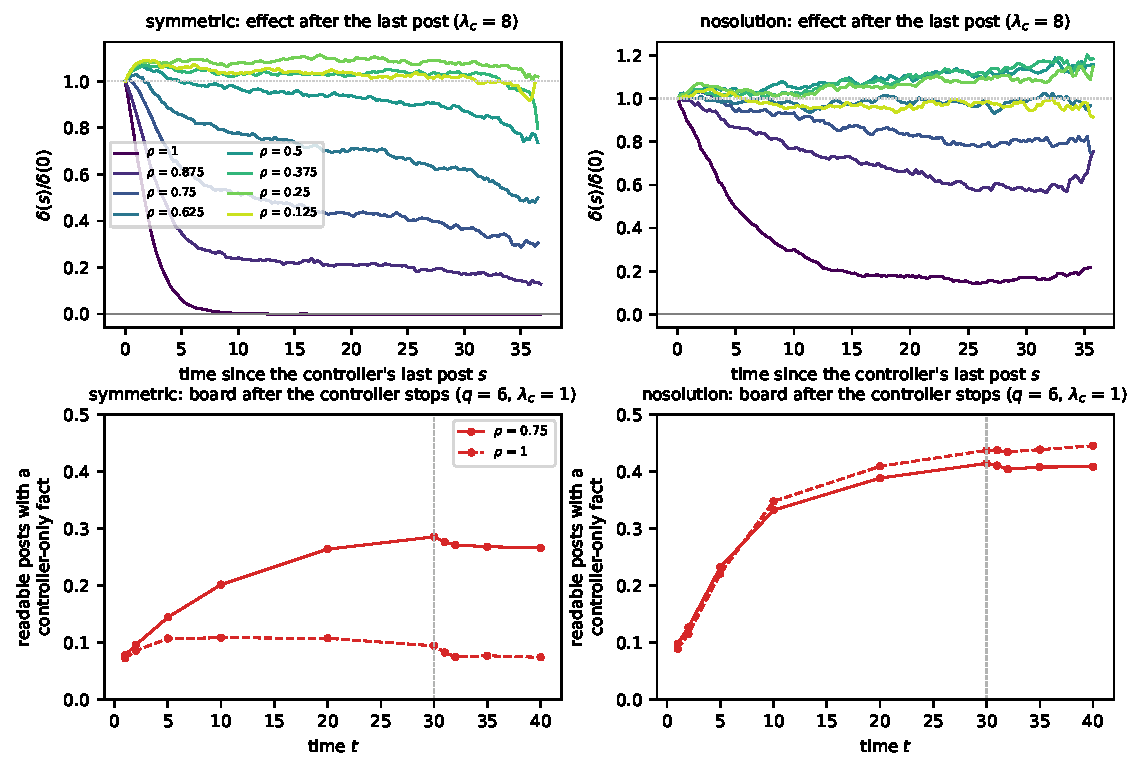
\includegraphics[width=0.95\linewidth]{fig3_persistence.pdf}
\caption{Top: $\delta(s)/\delta(0)$ after each episode's last post, $\lambda_c = 8$ (median $t^*$ 4--6 symmetric,
9--10 nosolution), one line per $\rho$; censored at $t = 40$. Bottom: readable posts with a controller-only fact,
false arm, $q = 6$, $\lambda_c = 1$.}
\label{fig:pers}
\end{figure}

\begin{itemize}\itemsep1pt
\item For $\rho \le 0.5$ the effect does not decay for more than 35 time units after the last post, in both tasks
  ($\delta(30)/\delta(0) = 0.87$--$1.14$); an unread fact's half-life is 0.3--1 time unit.
\item At higher memory it relaxes partly to a plateau: symmetric $\rho = 0.75$ to about 0.37 (half-time 11.5),
  nosolution $\rho = 1$ to about 0.17 (half-time 5). Whether the plateaus are permanent is unknown (no data beyond
  $t = 40$).
\item With a proof and full memory the effect vanishes within 2 time units.
\item From $t = 30$ to 40 the controller-only share of readable posts hardly changes (nosolution $\rho = 0.75$:
  0.41 $\to$ 0.41): agents keep reposting the controller's facts.
\end{itemize}

%-----------------------------------------------------------------------------------------------------------------------
\section{Backfire (secondary)}

\begin{figure}[H]
\centering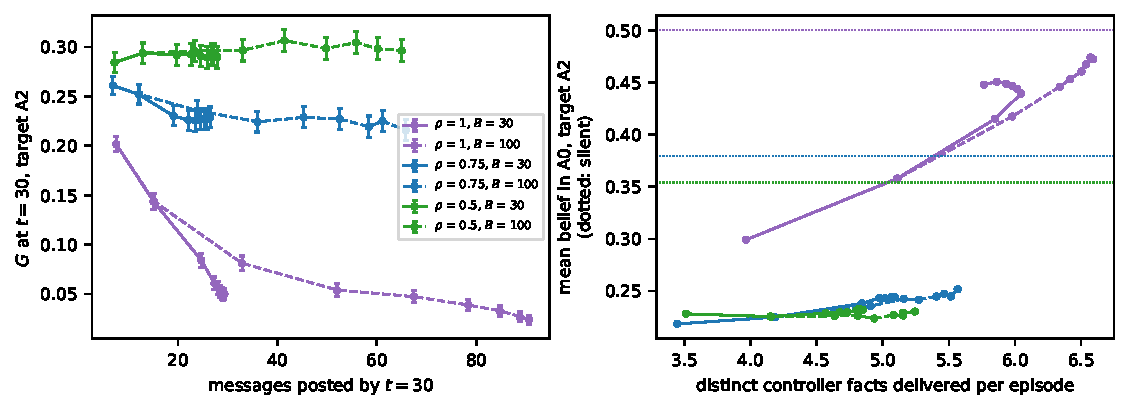
\includegraphics[width=0.95\linewidth]{fig6_backfire.pdf}
\caption{Nosolution, $q = 6$, gate on, $t = 30$, budgets 30 (solid) and 100 (dashed), rates 0.5--8. Left: $G$
against messages posted. Right: the false arm's mean belief in A0 against distinct controller facts delivered
(dotted: silent arm).}
\label{fig:backfire}
\end{figure}

\begin{itemize}\itemsep1pt
\item At $\rho = 1$, more messages lower $G$ (0.20 $\to$ 0.02 at 91 messages) as agents' belief in A0 returns toward
  the silent 0.50 (0.30 $\to$ 0.47).
\item At $\rho = 0.75$ the backfire is weak (0.26 $\to$ 0.22); at $\rho = 0.5$ $G$ is flat in messages.
\end{itemize}

\paragraph{Open.} Why reading protects (memory composition across $q$ at $\rho \le 0.5$: step 2) and what carries
the persistence (facts, biased state or communication: step 3).

\end{document}
